\documentclass[]{book}
\usepackage{lmodern}
\usepackage{amssymb,amsmath}
\usepackage{ifxetex,ifluatex}
\usepackage{fixltx2e} % provides \textsubscript
\ifnum 0\ifxetex 1\fi\ifluatex 1\fi=0 % if pdftex
  \usepackage[T1]{fontenc}
  \usepackage[utf8]{inputenc}
\else % if luatex or xelatex
  \ifxetex
    \usepackage{mathspec}
  \else
    \usepackage{fontspec}
  \fi
  \defaultfontfeatures{Ligatures=TeX,Scale=MatchLowercase}
\fi
% use upquote if available, for straight quotes in verbatim environments
\IfFileExists{upquote.sty}{\usepackage{upquote}}{}
% use microtype if available
\IfFileExists{microtype.sty}{%
\usepackage{microtype}
\UseMicrotypeSet[protrusion]{basicmath} % disable protrusion for tt fonts
}{}
\usepackage[margin=1in]{geometry}
\usepackage{hyperref}
\hypersetup{unicode=true,
            pdftitle={Machine Learning},
            pdfauthor={Mohamad Ghassany},
            pdfborder={0 0 0},
            breaklinks=true}
\urlstyle{same}  % don't use monospace font for urls
\usepackage{natbib}
\bibliographystyle{apalike}
\usepackage{longtable,booktabs}
\usepackage{graphicx,grffile}
\makeatletter
\def\maxwidth{\ifdim\Gin@nat@width>\linewidth\linewidth\else\Gin@nat@width\fi}
\def\maxheight{\ifdim\Gin@nat@height>\textheight\textheight\else\Gin@nat@height\fi}
\makeatother
% Scale images if necessary, so that they will not overflow the page
% margins by default, and it is still possible to overwrite the defaults
% using explicit options in \includegraphics[width, height, ...]{}
\setkeys{Gin}{width=\maxwidth,height=\maxheight,keepaspectratio}
\IfFileExists{parskip.sty}{%
\usepackage{parskip}
}{% else
\setlength{\parindent}{0pt}
\setlength{\parskip}{6pt plus 2pt minus 1pt}
}
\setlength{\emergencystretch}{3em}  % prevent overfull lines
\providecommand{\tightlist}{%
  \setlength{\itemsep}{0pt}\setlength{\parskip}{0pt}}
\setcounter{secnumdepth}{5}
% Redefines (sub)paragraphs to behave more like sections
\ifx\paragraph\undefined\else
\let\oldparagraph\paragraph
\renewcommand{\paragraph}[1]{\oldparagraph{#1}\mbox{}}
\fi
\ifx\subparagraph\undefined\else
\let\oldsubparagraph\subparagraph
\renewcommand{\subparagraph}[1]{\oldsubparagraph{#1}\mbox{}}
\fi

%%% Use protect on footnotes to avoid problems with footnotes in titles
\let\rmarkdownfootnote\footnote%
\def\footnote{\protect\rmarkdownfootnote}

%%% Change title format to be more compact
\usepackage{titling}

% Create subtitle command for use in maketitle
\newcommand{\subtitle}[1]{
  \posttitle{
    \begin{center}\large#1\end{center}
    }
}

\setlength{\droptitle}{-2em}
  \title{Machine Learning}
  \pretitle{\vspace{\droptitle}\centering\huge}
  \posttitle{\par}
  \author{Mohamad Ghassany}
  \preauthor{\centering\large\emph}
  \postauthor{\par}
  \predate{\centering\large\emph}
  \postdate{\par}
  \date{2016-12-14}

\usepackage{booktabs}

\begin{document}
\maketitle

{
\setcounter{tocdepth}{2}
\tableofcontents
}
\chapter*{Welcome}\label{welcome}
\addcontentsline{toc}{chapter}{Welcome}

Welcome to this course. It is only a little introduction to Machine
Learning.

The aim of Machine Learning is to build computer systems that can adapt
to their environments and learn form experience. Learning techniques and
methods from this field are successfully applied to a variety of
learning tasks in a broad range of areas, including, for example, spam
recognition, text classification, gene discovery, financial forecasting.
The course will give an overview of many concepts, techniques, and
algorithms in machine learning, beginning with topics such as linear
regression and classification and ending up with topics such as kmeans
and Expectation Maximization. The course will give the student the basic
ideas and intuition behind these methods, as well as a more formal
statistical and computational understanding. Students will have an
opportunity to experiment with machine learning techniques in R and
apply them to a selected problem.

\chapter*{Introduction}\label{introduction}
\addcontentsline{toc}{chapter}{Introduction}

\section*{What is Machine Learning ?}\label{what-is-machine-learning}
\addcontentsline{toc}{section}{What is Machine Learning ?}

What is Machine Learning?

Two definitions of Machine Learning are offered. Arthur Samuel described
it as: ``the field of study that gives computers the ability to learn
without being explicitly programmed.'' This is an older, informal
definition.

Tom Mitchell provides a more modern definition: ``A computer program is
said to learn from experience E with respect to some class of tasks T
and performance measure P, if its performance at tasks in T, as measured
by P, improves with experience E.''

Machine Learning is also called Statistical Learning.

Example: playing checkers.

E = the experience of playing many games of checkers

T = the task of playing checkers.

P = the probability that the program will win the next game.

In general, any machine learning problem can be assigned to one of two
broad classifications:

Supervised learning and Unsupervised learning.

\section*{Supervised Learning}\label{supervised-learning}
\addcontentsline{toc}{section}{Supervised Learning}

Supervised Learning is probably the most common type of machine learning
problem. Let's start with an example of what is it. Let's say we want to
predict housing prices. We plot a data set and it looks like this.

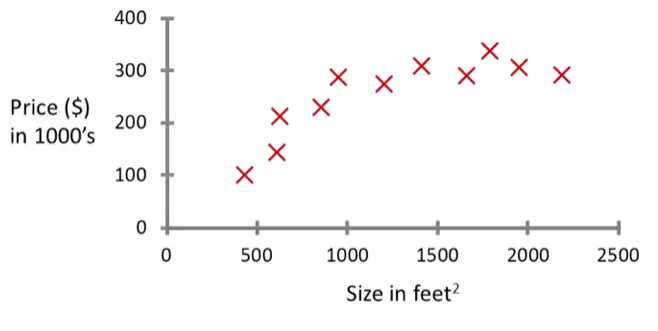
\includegraphics{img/sl1.png}

Here on the horizontal axis, the size of different houses in square
feet, and on the vertical axis, the price of different houses in
thousands of dollars.

So. Given this data, let's say we own a house that is, say 750 square
feet and hoping to sell the house and they want to know how much they
can get for the house.

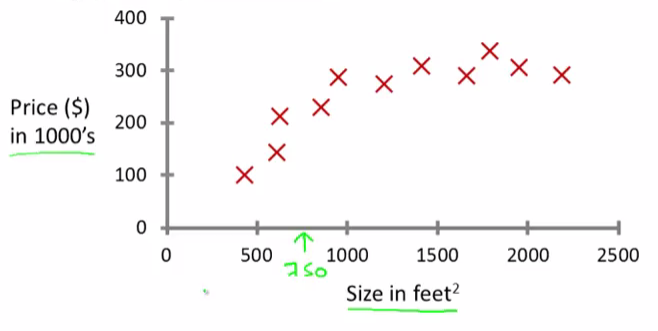
\includegraphics{img/sl2.png}

So how can the learning algorithm help?

One thing a learning algorithm might be able to do is put a straight
line through the data or to \textbf{``fit''} a straight line to the data
and, based on that, it looks like maybe the house can be sold for maybe
about \$150,000.

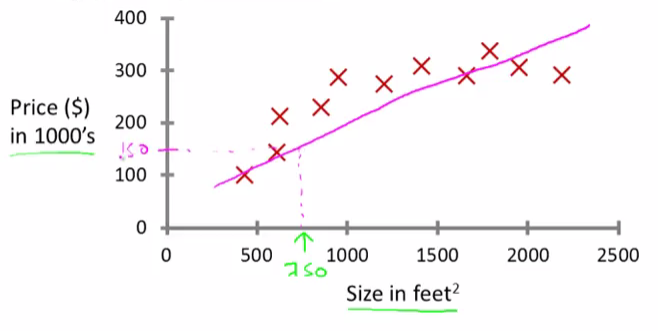
\includegraphics{img/sl3.png}

But maybe this isn't the only learning algorithm we can use. There might
be a better one. For example, instead of sending a straight line to the
data, we might decide that it's better to fit a \emph{quadratic
function} or a \emph{second-order polynomial} to this data.

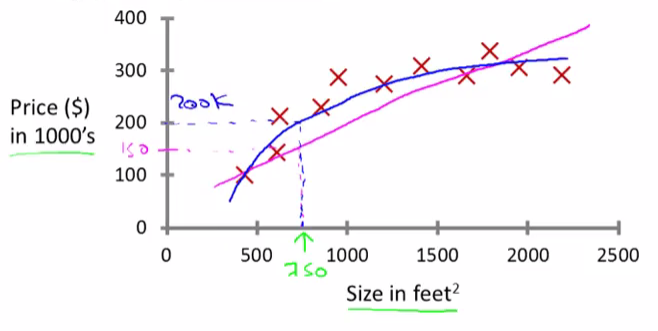
\includegraphics{img/sl4.png}

If we do that, and make a prediction here, then it looks like, well,
maybe we can sell the house for closer to \$200,000.

This is an example of a supervised learning algorithm.

The term supervised learning refers to the fact that we gave the
algorithm a data set in which the \textbf{``right answers''} were given.

The example above is also called a regression problem. A regression
problem is when we try to predict a \textbf{continuous} value output.
Namely the price in the example.

Here's another supervised learning example. Let's say we want to look at
medical records and try to predict of a breast cancer as malignant or
benign. If someone discovers a breast tumor, a lump in their breast, a
malignant tumor is a tumor that is harmful and dangerous and a benign
tumor is a tumor that is harmless. Let's see a collected data set and
suppose in the data set we have the size of the tumor on the horizontal
axis and on the vertical axis we plot one or zero, yes or no, whether or
not these are examples of tumors we've seen before are malignant (which
is one) or zero if not malignant or benign.

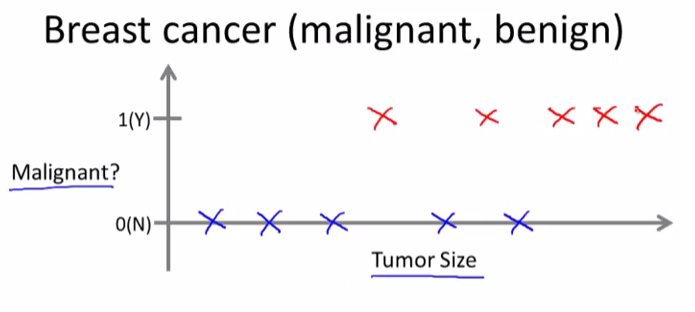
\includegraphics{img/sl5.png}

In this data set we have five examples of benign tumors, and five
examples of malignant tumors.

Let's say a person who tragically has a breast tumor, and let's say her
breast tumor size is known (rose arrow in the following figure).

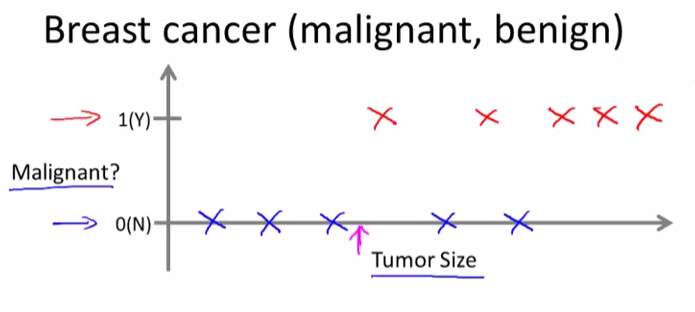
\includegraphics{img/sl6.png}

The machine learning question is, can you estimate what is the
probability that a tumor is malignant versus benign? To introduce a bit
more terminology this is an example of a classification problem.

The term classification refers to the fact that here we're trying to
predict a \textbf{discrete} value output: zero or one, malignant or
benign. And it turns out that in classification problems sometimes you
can have more than two values for the two possible values for the
output.

In classification problems there is another way to plot this data. Let's
use a slightly different set of symbols to plot this data. So if tumor
size is going to be the attribute that we are going to use to predict
malignancy or benignness, we can also draw the data like this.

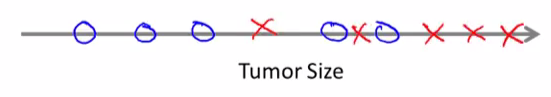
\includegraphics{img/sl7.png}

All we did was we took the data set on top and just mapped it down using
different symbols. So instead of drawing crosses, we are now going to
draw \texttt{O}'s for the benign tumors.

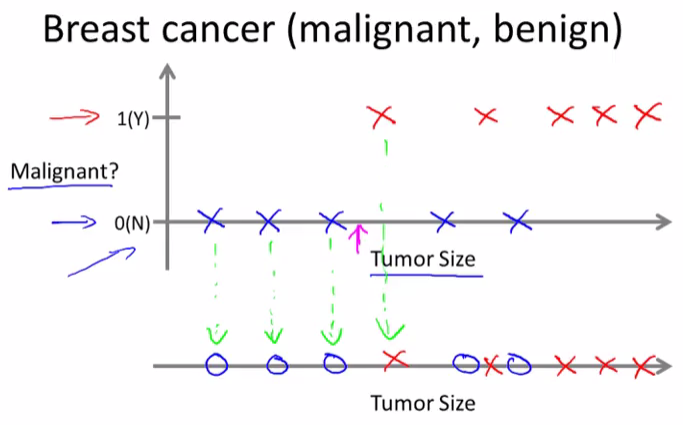
\includegraphics{img/sl8.png}

Now, in this example we use only one \textbf{feature} or one attribute,
mainly, the \emph{tumor size} in order to predict whether the tumor is
malignant or benign.

In other machine learning problems we may have more than one feature.

Here's an example. Let's say that instead of just knowing the tumor
size, we know both the age of the patients and the tumor size. In that
case maybe the data set will look like this.

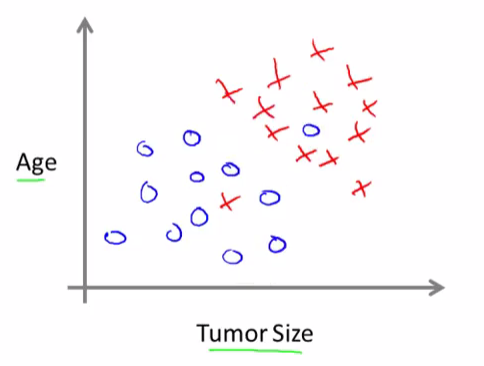
\includegraphics{img/sl9.png}

So, let's say a person who tragically has a tumor. And maybe, their
tumor size and age falls around there (rose point):

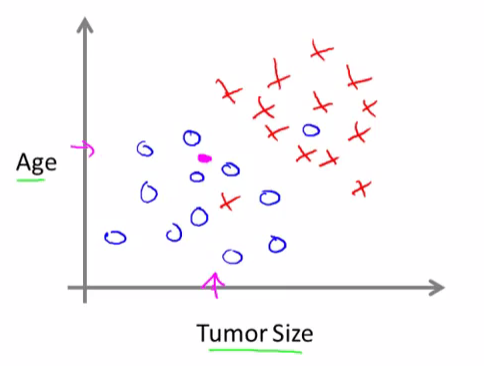
\includegraphics{img/sl10.png}

So given a data set like this, what the learning algorithm might do is
throw a straight line through the data to try to separate out the
malignant tumors from the benign ones. And with this, hopefully we can
decide that the person's tumor falls on this benign side and is
therefore more likely to be benign than malignant.

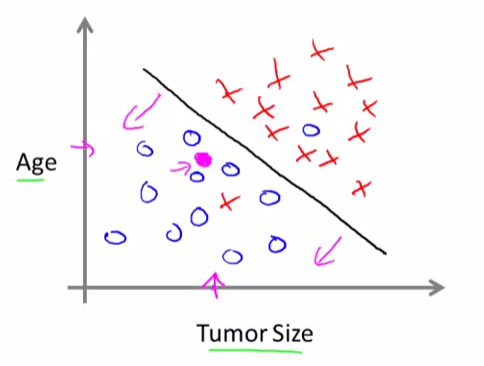
\includegraphics{img/sl11.png}

In this example we had \textbf{two features}, namely, the age of the
patient and the size of the tumor. In other machine learning problems we
will often have more features.

Most interesting learning algorithms is a learning algorithm that can
deal with, not just two or three or five features, but an
\textbf{infinite number of features}. So how do you deal with an
infinite number of features. How do you even store an infinite number of
things on the computer when your computer is gonna run out of memory.

\section*{Unsupervised Learning}\label{unsupervised-learning}
\addcontentsline{toc}{section}{Unsupervised Learning}

The second major type of machine learning problem is called Unsupervised
Learning.

The difference between Unsupervised Learning and Supervised Learning is
that in Supervised Learning we are told explicitly what is the so-called
right answers (data are labeled).

In Unsupervised Learning, we're given data that doesn't have any labels
or that all has the same label or really no labels. Like in this
example:

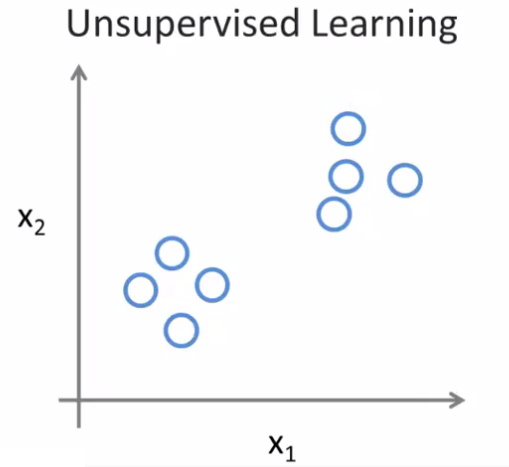
\includegraphics{img/ul1.png}

So we're given the data set and we're not told what to do with it and
we're not told what each data point is. Instead we're just told, here is
a data set. Can you find some structure in the data?

Given this data set, an Unsupervised Learning algorithm might decide
that the data lives in two different clusters.

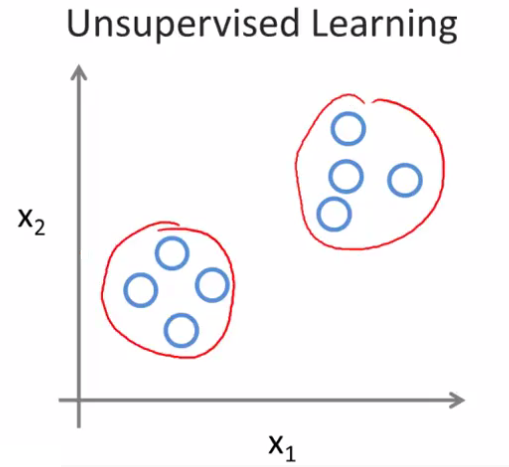
\includegraphics{img/ul2.png}

This is called a \textbf{clustering} algorithm.

Here are two examples where Unsupervised Learning or clustering is used.

Social network analysis:

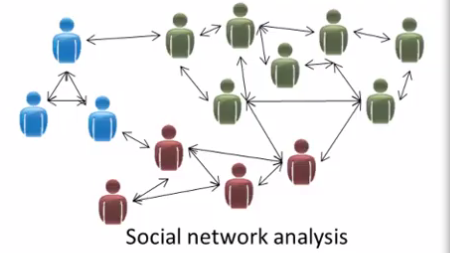
\includegraphics{img/ul3.png}

So given knowledge about which friends you email the most or given your
Facebook friends or your Google+ circles, can we automatically identify
which are cohesive groups of friends, also which are groups of people
that all know each other?

Market segmentation:

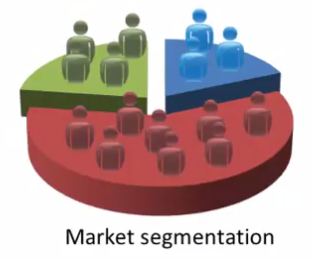
\includegraphics{img/ul4.png}

Many companies have huge databases of customer information. So, can you
look at this customer data set and automatically discover market
segments and automatically group your customers into different market
segments so that you can automatically and more efficiently sell or
market your different market segments together?

This is Unsupervised Learning because we have all this customer data,
but we don't know in advance what are the market segments and for the
customers in our data set, we don't know in advance who is in market
segment one, who is in market segment two, and so on. But we have to let
the algorithm discover all this just from the data.

◼

\part{Supervised Learning}\label{part-supervised-learning}
\addcontentsline{toc}{chapter}{(PART) Supervised Learning}

\part{Regression}\label{part-regression}
\addcontentsline{toc}{chapter}{(PART) Regression}

\chapter{Linear Regression}\label{linear-regression}

\section{Notation}\label{notation}

In general, we will let \(x_{ij}\) represent the value of the \(j\)th
variable for the \(i\)th observation, where \(i=1,2,\ldots,n\) and
\(j=1,2,\ldots,p\). We will use \(i\) to index the samples or
observations (from \(1\) tp \(n\)) and \(j\) will be used to index the
variables (or features) (from \(1\) to \(p\)). We let \(\textbf{X}\)
denote a \(n \times p\) matrix whose \((i,j)\)th element is \(x_{ij}\).
That is,

\[ \textbf{X}  = \begin{pmatrix}
    x_{11} & x_{12} & x_{13} & \dots  & x_{1p} \\
    x_{21} & x_{22} & x_{23} & \dots  & x_{2p} \\
    \vdots & \vdots & \vdots & \ddots & \vdots \\
    x_{n1} & x_{n2} & x_{n3} & \dots  & x_{np}
\end{pmatrix} \]

Note that it is useful to visualize \(\textbf{X}\) as a spreadsheet of
numbers with \(n\) rows and \(p\) columns. We will write the rows of
\(\textbf{X}\) as \(x_1 , x_2 , \ldots, x_n\). Here \(x_i\) is a vector
of length \(p\), containing the \(p\) variable measurements for the
\(i\)th observation. That is,

\[ x_i = \begin{pmatrix}
    x_{i1} \\
    x_{i2} \\
    \vdots \\
    x_{ip}
\end{pmatrix}\]

(Vectors are by default represented as columns.)

We will write the columns of \(\textbf{X}\) as
\(\textbf{x}_1 , \textbf{x}_2, \ldots, \textbf{x}_p\). Each is a vector
of length \(n\). That is,

\[ \textbf{x}_j = \begin{pmatrix}
    \textbf{x}_{1j} \\
    \textbf{x}_{2j} \\
    \vdots \\
    \textbf{x}_{nj}
\end{pmatrix}\]

Using this notation, the matrix \(\textbf{X}\) can be written as

\[ \textbf{X} = (\textbf{x}_1  \textbf{x}_2 \ldots \textbf{x}_p) \]

or

\[ \textbf{X} = \begin{pmatrix}
    x_{1}^T \\
    x_{2}^T \\
    \vdots \\
    x_{n}^T
\end{pmatrix}\]

The \(^T\) notation denotes the transpose of a matrix or vector.

We use \(y_i\) to denote the \(i\)th observation of the variable on
which we wish to make predictions. We write the set of all \(n\)
observations in vector form as

\[ \textbf{y} = \begin{pmatrix}
    y_{1}^T \\
    y_{2}^T \\
    \vdots \\
    y_{n}^T
\end{pmatrix}\]

Then the observed data consists of
\(\{(x_1, y_1), (x_2 , y_2 ), \ldots , (x_n , y_n )\}\), where each
\(x_i\) is a vector of length \(p\). (If \(p = 1\), then \(x_i\) is
simply a scalar).

\section{Model Representation}\label{model-representation}

Let's consider the example about predicting housing prices. We're going
to use this data set as an example,

\begin{figure}[htbp]
\centering
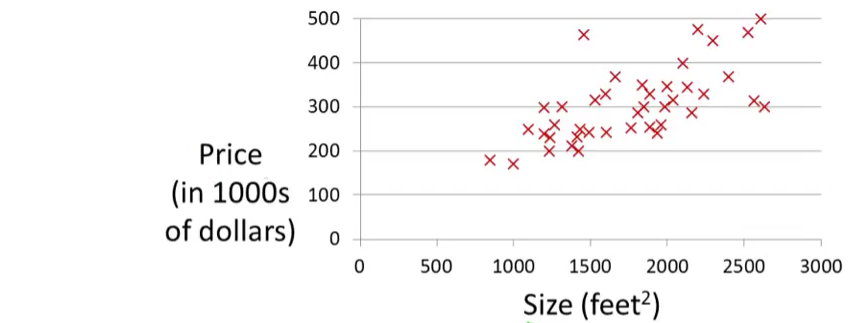
\includegraphics{img/mr1.png}
\caption{}
\end{figure}

Suppose that there is a person trying to sell a house of size 1250
square feet and he wants to know how much he might be able to sell the
house for. One thing we could do is fit a model. Maybe fit a straight
line to this data. Looks something like this,

\begin{figure}[htbp]
\centering
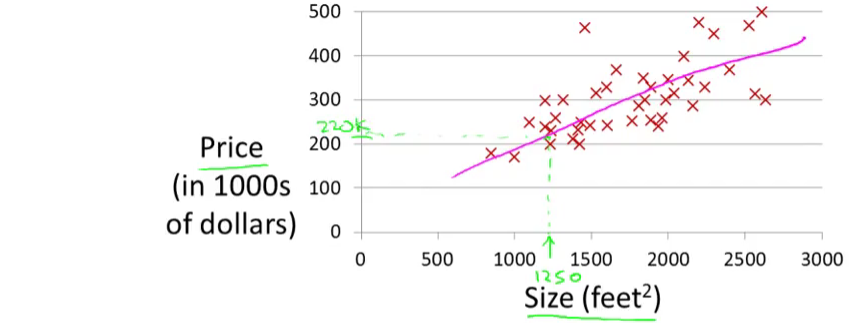
\includegraphics{img/mr2.png}
\caption{}
\end{figure}

and based on that, maybe he can sell the house for around \$220,000.
Recall that this is an example of a supervised learning algorithm. And
it's supervised learning because we're given the ``right answer'' for
each of our examples. More precisely, this is an example of a regression
problem where the term regression refers to the fact that we are
predicting a real-valued output namely the price.

More formally, in supervised learning, we have a data set and this data
set is called a \textbf{training set}. So for housing prices example, we
have a training set of different housing prices and our job is to learn
from this data how to predict prices of the houses.

Let's define some notation from this data set:

\begin{itemize}
\tightlist
\item
  The size of the house is the input variable.
\item
  The house price is the output variable.
\item
  The input variables are typically denoted using the variable symbol
  \(X\),
\item
  The inputs go by different names, such as \emph{predictors},
  \emph{independent variables}, \emph{features}, \emph{predictor} or
  sometimes just \emph{variables}.
\item
  The output variable is often called the \emph{response},
  \emph{dependent variable} or \emph{target}, and is typically denoted
  using the symbol \(Y\).
\item
  \((x_i,y_i)\) is the \(i\)th training example.
\item
  The set of \(\{(x_i, y_i)\}\) is the training set.
\item
  \(n\) is the number of training examples.
\end{itemize}

So here's how this supervised learning algorithm works. Suppose that we
observe a quantitative response \(Y\) and \(p\) different predictors,
\(X_1 , X_2 ,\ldots, X_p\) . We assume that there is some relationship
between \(Y\) and \(X = (X_1 , X_2 ,\ldots, X_p)\), which can be written
in the very general form

\[Y = f(X) + \epsilon\]

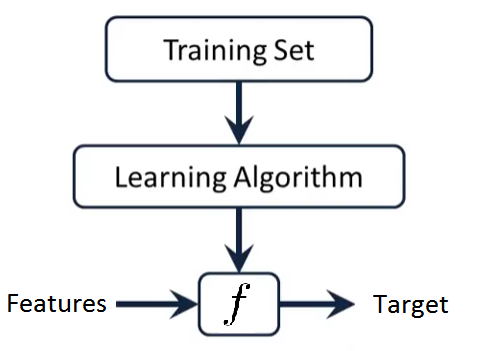
\includegraphics{img/mr3.png}

Here \(f\) is some fixed but unknown function of
\(X_1 , X_2 ,\ldots, X_p\) , and \(\epsilon\) is a random error term,
which is independent of \(X\) and has mean zero. The \(f\) function is
also called \emph{hypothesis} in Machine Learning. In general, the
function \(f\) may involve more than one input variable. In essence,
Supervised Learning refers to a set of approaches for estimating \(f\).

\section{\texorpdfstring{Why Estimate \(f\)
?}{Why Estimate f ?}}\label{why-estimate-f}

There are two main reasons that we may wish to estimate \(f\):
\emph{prediction} and \emph{inference}.

\subsection*{Prediction}\label{prediction}
\addcontentsline{toc}{subsection}{Prediction}

In many situations, a set of inputs \(X\) are readily available, but the
output \(Y\) cannot be easily obtained. In this setting, since the error
term averages to zero, we can predict \(Y\) using

\[ \hat{Y} = \hat{f}(X) \]

where \(\hat{f}\) represents our estimate for \(f\), and \(\hat{Y}\)
represents the resulting prediction for \(Y\). Like in the example above
about predicting housing prices.

We can measure the accuracy of \(\hat{Y}\) by using a \textbf{cost
function}. In the regression models, the most commonly-used measure is
the \emph{mean squared error} (MSE), given by

\[ MSE = \frac{1}{n} \sum_{i=1}^{n} (y_i - \hat{f}(x_i))^2\]

\subsection*{Inference}\label{inference}
\addcontentsline{toc}{subsection}{Inference}

We are often interested in understanding the way that \(Y\) is affected
as \(X_1 , X_2 ,\ldots, X_p\) change. In this situation we wish to
estimate \(f\) , but our goal is not necessarily to make predictions for
\(Y\). We instead want to understand the relationship between \(X\) and
\(Y\), or more specifically, to understand how \(Y\) changes as a
function of \(X_1 , X_2 ,\ldots, X_p\). In this case, one may be
interested in answering the following questions:

\begin{itemize}
\tightlist
\item
  Which predictors are associated with the response?
\item
  What is the relationship between the response and each predictor?
\item
  Can the relationship between Y and each predictor be adequately
  summarized using a linear equation, or is the relationship more
  complicated?
\end{itemize}

\section{Simple Linear Regression}\label{simple-linear-regression}

\subsection{Model}\label{model}

\emph{Simple linear regression} is a very straightforward approach for
predicting a quantitative response \(Y\) on the basis of a single
predictor variable \(X\). It assumes that there is approximately a
linear relationship between \(X\) and \(Y\). Mathematically, we can
write this linear relationship as

\[ Y = \beta_0 + \beta_1 X + \epsilon \]
\[Y \approx \beta_0 + \beta_1 X\]

where \(\beta_0\) and \(\beta_1\) are two unknown constants that
represent the \emph{intercept} and \emph{slope}, also known as
\textbf{\emph{coefficients}} or \emph{parameters}, and \(\epsilon\) is
the error term.

Given some estimates \(\hat{\beta_0}\) and \(\hat{\beta_1}\) for the
model coefficients, we predict future inputs \(x\) using

\[\hat{y} = \hat{\beta_0} + \hat{\beta_1} x\]

where \(\hat{y}\) indicates a prediction of \(Y\) on the basis of
\(X = x\). The \emph{hat} symbol, \(\hat{}\), denotes an estimated
value.

\subsection{Estimating the
Coefficients}\label{estimating-the-coefficients}

Let \(\hat{y}_i = \hat{\beta_0} + \hat{\beta_1} x_i\) be the prediction
for \(Y\) based on the \(i\)th value of \(X\). Then
\(e_i = y_i - \hat{y}_i\) represents the \(i\)th
\textbf{\emph{residual}}.

We define the \textbf{\emph{residual sum of squares}} (\textbf{RSS}) as

\[  \begin{aligned}
RSS &= e_1^2 + e_2^2 + \ldots + e_n^2 \\
    &= \sum_{i=1}^{n} e_i^2
 \end{aligned}  \]

or equivantly as

\[ \begin{aligned}
RSS &= (y_1 - \hat{\beta_0} - \hat{\beta_1} x_1)^2 + (y_2 - \hat{\beta_0} - \hat{\beta_1} x_2)^2 + \ldots + (y_n - \hat{\beta_0} - \hat{\beta_1} x_n)^2 \\
    &= \sum_{i=1}^{n} (y_i - \hat{\beta_0} - \hat{\beta_1} x_i)^2
\end{aligned} \]

The \emph{least squares} approach chooses \(\hat{\beta_0}\) and
\(\hat{\beta_1}\) to minimize the RSS. The minimizing values can be show
to be

\[  \begin{aligned}
\hat{\beta_1} &=  \frac{\sum_{i=1}^{n} (x_i - \bar{x})(y_i - \bar{y})  }{\sum_{i=1}^{n} (x_i - \bar{x})^2 } \\
\text{and} \\
\hat{\beta_0} &= \bar{y} - \hat{\beta_1} \bar{x}
\end{aligned}  \]

where \(\bar{y} = \frac{1}{n} \sum_{i=1}^{n} y_i\) and
\(\bar{x} = \frac{1}{n} \sum_{i=1}^{n} x_i\) are the sample means.

\subsection{Assessing the Accuracy of the Coefficient
Estimates}\label{assessing-the-accuracy-of-the-coefficient-estimates}

The standard error of an estimator reflects how it varies under repeated
sampling. We have

\[ \text{SE}(\hat{\beta_1})^2 =  \frac{\sigma^2}{\sum_{i=1}^{n} (x_i - \bar{x})^2} \]

\[ \text{SE}(\hat{\beta_0})^2 = \sigma^2 \bigg[ \frac{1}{n} +  \frac{\bar{x}^2}{\sum_{i=1}^{n} (x_i - \bar{x})^2} \bigg] \]

where \(\sigma^2 = Var(\epsilon)\)

In general, \(\sigma^2\) is know known, but can be estimated from the
data. The estimate of \(\sigma\) is known as the \emph{residual standard
error}, and is given by

\[ \text{RSE} = \sqrt{\frac{\text{RSS}}{(n-2)}} \]

These standard errors can be used to compute \emph{confidence
intervals}. A \(95\%\) confidence interval is defined as a range of
values such that with \(95\%\) probability, the range will contain the
true unknown value of the parameter. It has the form

\[ \hat{\beta_1} \pm 2 \cdot \text{SE}(\hat{\beta_1}) \]

That is, there is approximately a \(95\%\) chance that the interval

\[ \bigg[  \hat{\beta_1} - 2 \cdot \text{SE}(\hat{\beta_1}), \hat{\beta_1} + 2 \cdot \text{SE}(\hat{\beta_1})   \bigg] \]

will contain the true value of \(\beta_1\). Similarly, a confidence
interval for \(\beta_0\) approximately takes the form

\[ \hat{\beta_0} \pm 2 \cdot \text{SE}(\hat{\beta_0}) \]

\subsubsection*{Hypothesis testing}\label{hypothesis-testing}
\addcontentsline{toc}{subsubsection}{Hypothesis testing}

Standard errors can also be used to perform \emph{hypothesis tests} on
the coefficients. The most common hypothesis test involves testing the
\emph{null hypothesis} of

\[ H_0 : \text{There is no relationship between} \, X \, \text{and} \, Y \]

versus the \emph{alternative hypothesis}

\[ H_1 : \text{There is some relationship between} \, X \, \text{and} \, Y \]

Mathematically, this corresponds to testing

\[ H_0 : \beta_1 = 0 \]

versus

\[ H_1 : \beta_1 \neq 0 \]

since if \(\beta_1 = 0\) then the simple linear regression model reduces
to \(Y = \beta_0 + \epsilon\), and \(X\) is not associated with \(Y\).

To test the null hypothesis \(H_0\), we compute a
\textbf{\emph{t-statistic}}, given by

\[ t = \frac{\hat{\beta_1} - 0}{\text{SE}(\hat{\beta_1})} \]

This will have a \(t\)-distribution (\emph{Student}) with \(n-2\)
degrees of freedom, assuming \(\beta_1=0\).

Using statistical software, it is easy to compute the probability of
observing any value equal to \(|t|\) or larger. We call this probability
the \textbf{\emph{p-value}}.

If p-value is small enough (typically under \(0.01\) (\(1\%\) error) or
\(0.05\) (\(5\%\) error)) we reject the null hypothesis, that is we
declare a relationship to exist between \(X\) and \(Y\).

\subsection{Assessing the Accuracy of the
Model}\label{assessing-the-accuracy-of-the-model}

Once we have rejected the null hypothesis in favor of the alternative
hypothesis, it is natural to want to quantify the extent to which the
model fits the data. The quality of a linear regression fit is typically
assessed using two related quantities: the \emph{residual standard
error} (RSE) and the \(R^2\) statistic.

\subsubsection*{Residual Standard Error
(RSE)}\label{residual-standard-error-rse}
\addcontentsline{toc}{subsubsection}{Residual Standard Error (RSE)}

The Residual Standard Error (RSE) is computed using the formula

\[ \text{RSE} = \sqrt{\frac{\text{RSS}}{(n-2)}} =  \sqrt{\frac{ \sum_{i=1}^{n} (y_i - \hat{y}_i)^2 }{(n-2)}} \]

recall that RSS is the \emph{residual sum-of-squares}.

The RSE is considered a measure of the lack of fit of the model to the
data. If the predictions obtained using the model are very close to the
true outcome values (if \(\hat{y}_i = y_i\) for \(i = 1, \ldots, n\))
then RSE will be small, and we can conclude that the model fits the data
very well. On the other hand, if \(\hat{y}_i\) is very far from \(y_i\)
for one or more observations, then the RSE may be quite large,
indicating that the model doesn't fit the data well.

\subsubsection*{\texorpdfstring{\(R^2\)
Statistic}{R\^{}2 Statistic}}\label{r2-statistic}
\addcontentsline{toc}{subsubsection}{\(R^2\) Statistic}

To calculate \(R^2\), we use the formula

\[ R^2 = \frac{\text{TSS} - \text{RSS}}{\text{TSS}} = 1- \frac{\text{RSS}}{\text{TSS}} \]

where \(\text{TSS} = \sum (y_i - \bar{y})^2\) is the \emph{total sum of
squared}.

\(R^2\) measures the \emph{proportion of variability in} \(Y\)
\emph{that can be explained using} \(X\). An \(R^2\) statistic that is
close to 1 indicates that a large proportion of the variability in the
response has been explained by the regression. A number near 0 indicates
that the regression did not explain much of the variability in the
response; this might occur because the linear model is wrong, or the
inherent error \(\sigma^2\) is high, or both.

It can be shown that in this simple linear linear regression setting
that \(R^2 = r^2\), where \(r\) is the correlation between \(X\) and
\(Y\):

\[ r = \frac{cov(X,Y)}{\sigma_X \sigma_Y} \]

◼

\chapter*{PW 1}\label{pw-1}
\addcontentsline{toc}{chapter}{PW 1}

\subsection*{~How to use R}\label{how-to-use-r}
\addcontentsline{toc}{subsection}{~How to use R}

Rstudio

intro to r from \textasciitilde{}macro \textbf{NO} intro R Julien
jacques \textbf{Maybe?} or intro to R from tibshirani's book
\textbf{Maybe?}
\href{https://cran.r-project.org/doc/contrib/Torfs+Brauer-Short-R-Intro.pdf}{A
(very) short introduction to R} \textbf{Maybe?}

Data preprocessing from udemy

Markdown Rmarkdown Html notebook

\subsection*{Get familiar with R}\label{get-familiar-with-r}
\addcontentsline{toc}{subsection}{Get familiar with R}

Notions

Data preprocessing from udemy

\subsection*{~Linear Regression}\label{linear-regression-1}
\addcontentsline{toc}{subsection}{~Linear Regression}

Application on the salary example from udemy or Abass el sharif ready
pdf

\chapter{Multiple Linear Regression}\label{multiple-linear-regression}

Simple linear regressionis a useful approach for predicting a response
on the basis of a single predictor variable. However, in practice we
often have more than one predictor. In the previous chapter, we took for
example the prediction of housing prices considering we had the size of
each house. We had a single feature \(X\), the size of the house. But
now imagine if we had not only the size of the house as a feature but we
also knew the number of bedrooms, the number of flours and the age of
the home in years. It seems like this would give us a lot more
information with which to predict the price.

\section{The Model}\label{the-model}

In general, suppose that we have p distinct predictors. Then the
multiple linear regression model takes the form

\[ Y = \beta_0 + \beta_1 X_1 + \beta_2 X_2 + \dots + \beta_p X_p + \epsilon \]

where \(X_j\) represents the \(j\)th predictor and \(\beta_j\)
quantifies the association between that variable and the response. We
interpret \(\beta_j\) as the average effect on \(Y\) of a one unit
increase in \(X_j\), \emph{holding all other predictors fixed}.

In matrix terms, supposing we have \(n\) observations and \(p\)
variables, we need to define the following matrices:

\begin{equation}
 \textbf{Y}_{n \times 1} = \begin{pmatrix}
    Y_{1} \\
    Y_{2} \\
    \vdots \\
    Y_{n}
\end{pmatrix}   \,\,\,\,\,\,\,\,\,\,\,\,  \textbf{X}_{n \times (p+1)}  = \begin{pmatrix}
    1      & X_{11} & X_{12} & \dots  & X_{1p} \\
    1      & X_{21} & X_{22} & \dots  & X_{2p} \\
    \vdots & \vdots & \vdots & \ddots & \vdots \\
    1      & X_{n1} & X_{n2} & \dots  & X_{np}
\end{pmatrix}
\end{equation}

\begin{equation}
 {\mathbb{\beta}}_{(p+1) \times 1} = \begin{pmatrix}
    \beta_{0} \\
    \beta_{1} \\
    \vdots \\
    \beta_{p}
    \end{pmatrix}   \,\,\,\,\,\,\,\,\,\,\,\,  {\epsilon}_{n \times 1} = \begin{pmatrix}
        \epsilon_{1} \\
        \epsilon_{2} \\
        \vdots \\
        \epsilon_{n}
    \end{pmatrix}
\end{equation}

In matrix terms, the general linear regression model is

\[ \textbf{Y}_{n \times 1} = \textbf{X}_{n \times (p+1)} {\mathbb{\beta}}_{(p+1) \times 1} + {\epsilon}_{n \times 1} \]

where,

\begin{itemize}
\tightlist
\item
  \(\textbf{Y}\) is a vector of responses.
\item
  \(\mathbb{\beta}\) is a vector of parameters.
\item
  \(\textbf{X}\) is a matrix of constants.
\item
  \(\epsilon\) is a vector of independent normal random variables.
\end{itemize}

\section{Estimating the Regression
Coefficients}\label{estimating-the-regression-coefficients}

As was the case in the simple linear regression setting, the regression
coefficients \(\beta_{0}, \beta_{1}, \ldots, \beta_{p}\) are unknown,
and must be estimated. Given estimates
\(\hat{\beta_{0}}, \hat{\beta_{1}}, \ldots, \hat{\beta_{p}}\), we can
make predictions using the formula

\[ \hat{y} = \hat{\beta_{0}} + \hat{\beta_{1}} x_1 + \hat{\beta_{2}} x_2 + \ldots, \hat{\beta_{p}} x_p \]

We choose \(\beta_{0}, \beta_{1}, \ldots, \beta_{p}\) to minimize the
sum of squared residuals

\[ \begin{aligned}
RSS &= \sum_{i=1}^{n} (y_i - \hat{y}_i)^2 \\
    &= \sum_{i=1}^{n} (y_1 - \hat{\beta_0} - \hat{\beta_1} \hat{x}_{i1}  - \hat{\beta_2} \hat{x}_{i2} - \ldots  -  \hat{\beta_p} \hat{x}_{ip})^2 \\
\end{aligned}
\]

The values \(\hat{\beta_{0}}, \hat{\beta_{1}}, \ldots, \hat{\beta_{p}}\)
that minimize the RSS are the multiple least squares regression
coefficient estimates, they are calculated using this formula (in matrix
terms):

\[ \hat{\beta} = (\textbf{X}^T \textbf{X})^{-1}\textbf{X}^T \textbf{Y} \]

Note 1:

\begin{quote}
It is a remarkable property of matrix algebra that the results for the
general linear regression model in matrix notation appear exactly as
those for the simple linear regression model. Only the degrees of
freedom and other constants related to the number of \(X\) variables and
the dimensions of some matrices are different.
\end{quote}

Note 2:

\begin{quote}
If \(\textbf{X}^T \textbf{X}\) is noninvertible, the common causes might
be having:
\end{quote}

\begin{quote}
\begin{itemize}
\tightlist
\item
  Redundant features, where two features are very closely related
  (i.e.~they are linearly dependent)
\item
  Too many features (e.g. \(p \geq n\)). In this case, we delete some
  features or we use ``regularization'' (to be explained in a later
  lesson).
\end{itemize}
\end{quote}

\section{Some important questions}\label{some-important-questions}

When we perform multiple linear regression, we usually are interested in
answering a few important questions.

\begin{enumerate}
\def\labelenumi{\arabic{enumi}.}
\tightlist
\item
  Is at least one of the predictors \(X_1 ,X_2 ,\ldots,X_p\) useful in
  predicting the response?
\item
  Do all the predictors help to explain \(Y\), or is only a subset of
  the predictors useful?
\item
  How well does the model fit the data?
\item
  Given a set of predictor values, what response value should we
  predict, and how accurate is our prediction?
\end{enumerate}

\textbf{\emph{Relationship Between the Response and Predictors?}}

\textbf{\(F\)-Statistic}

Recall that in the simple linear regression setting, in order to
determine whether there is a relationship between the response and the
predictor we can simply check whether \(\beta_1 = 0\). In the multiple
regression setting with \(p\) predictors, we need to ask whether all of
the regression coefficients are zero, i.e.~whether
\(\beta_1 = \beta_2 = \ldots = \beta_p = 0\). As in the simple linear
regression setting, we use a hypothesis test to answer this question. We
test the null hypothesis,

\[ H_0 : \beta_1 = \beta_2 = \ldots = \beta_p = 0 \]

versus the alternative hypothesis

\[ H_1 : \text{at least one} \, \beta_j \, \text{is non-zero} \]

This hypothesis test is performed by computing the \(F\)-statistic
(\emph{Fisher}):

\[ F = \frac{ (\text{TSS} - \text{RSS})/p}{\text{RSS}/(n-p-1)} \sim F_{p,n-p-1} \]

where, as with simple linear regression,
\(\text{TSS} = \sum (y_i - \bar{y})^2\) and
\(\text{RSS} = \sum (y_i - \hat{y}_i)^2\).

When the \(F\)-statistic value is close to 1, then \(H_0\) is true,
which means there is no relationship between the response and
predictors. On the other hand, if \(H_1\) is true, so we expect \(F\) to
be greater than 1.

So the question we ask here: \emph{Is the whole regression explaining
anything at all?} The answer comes from the \(F\)-test in the ANOVA
(ANalysis Of VAriance) table. This is what we get in an ANOVA table:

\begin{longtable}[]{@{}llllll@{}}
\toprule
Source & df & SS & MS & \(F\) & p-value\tabularnewline
\midrule
\endhead
Factor (Explained) & \(p-1\) & SST & SST/\((k-1)\) & MST/MSE &
p-value\tabularnewline
Error (Unexplained) & \(n-p\) & SSE & SSE/\((n-k)\) & &\tabularnewline
Total & \(n-1\) & SS & & &\tabularnewline
\bottomrule
\end{longtable}

The ANOVA table has many pieces of information. What we care about is
the \(F\) Ratio and the corresponding p-value. We compare the \(F\)
Ratio with \(F_{(p-1,n-p)}\) and a corresponding \(\alpha\) value
(error).

\textbf{p-values}

The p-values provide information about whether each individual predictor
is related to the response, after adjusting for the other predictors.
Let's look at the following table we obtain in general using a
statistical software for example

\begin{longtable}[]{@{}lllll@{}}
\toprule
& Coefficient & Std. error & \(t\)-statistic & p-value\tabularnewline
\midrule
\endhead
Constant & 2.939 & 0.3119 & 9.42 & \textless{}0.0001\tabularnewline
\(X_1\) & 0.046 & 0.0014 & 32.81 & \textless{}0.0001\tabularnewline
\(X_2\) & 0.189 & 0.0086 & 21.89 & \textless{}0.0001\tabularnewline
\(X_3\) & -0.001 & 0.0059 & -0.18 & 0.8599\tabularnewline
\bottomrule
\end{longtable}

In this tablewe the following model

\[ Y = 2.939 + 0.046 X_1 + 0.189 X_2 - 0.001 X_3 \]

Note that for each individual predictor a \(t\)-statistic and a p-value
were reported. These p-values indicate that \(X_1\) and \(X_2\) are
related to \(Y\), but that there is no evidence that \(X_3\) is
associated with \(Y\), in the presence of these two.

\textbf{\emph{Deciding on Important Variables}}

The most direct approach is called \emph{all subsets} or \emph{best
subsets} regression: we compute the least squares fit for all possible
subsets and then choose between them based on some criterion that
balances training error with model size.

However we often can't examine all possible models, since they are
\(2^p\) of them; for example when \(p = 40\) there are over a billion
models! Instead we need an automated approach that searches through a
subset of them. Here are two commonly use approaches:

\textbf{Forward selection}:

\begin{itemize}
\tightlist
\item
  Begin with the \emph{null model} --- a model that contains an
  intercept (constant) but no predictors.
\item
  Fit p simple linear regressions and add to the null model the variable
  that results in the lowest RSS.
\item
  Add to that model the variable that results in the lowest RSS amongst
  all two-variable models.
\item
  Continue until some stopping rule is satisfied, for example when all
  remaining variables have a p-value above some threshold.
\end{itemize}

\textbf{Backward selection}:

\begin{itemize}
\tightlist
\item
  Start with all variables in the model.
\item
  Remove the variable with the largest p-value --- that is, the variable
  that is the least statistically significant.
\item
  The new \((p − 1)\)-variable model is fit, and the variable with the
  largest p-value is removed.
\item
  Continue until a stopping rule is reached. For instance, we may stop
  when all remaining variables have a significant p-value defined by
  some significance threshold.
\end{itemize}

\begin{quote}
There are more systematic criteria for choosing an ``optimal'' member in
the path of models produced by forward or backward stepwise selection.
These include \emph{Mallow's \(C_p\)} , \emph{Akaike information
criterion (AIC)}, \emph{Bayesian information criterion (BIC)},
\emph{adjusted \(R^2\)} and \emph{Cross-validation (CV)}.
\end{quote}

\textbf{\emph{Model Fit}}

Two of the most common numerical measures of model fit are the RSE and
\(R^2\), the fraction of variance explained. These quantities are
computed and interpreted in the same fashion as for simple linear
regression. Recall that in simple regression, \(R^2\) is the square of
the correlation of the response and the variable. In multiple linear
regression, it turns out that it equals \(Cor(Y, \hat{Y})^2\) , the
square of the correlation between the response and the fitted linear
model; in fact one property of the fitted linear model is that it
maximizes this correlation among all possible linear models. An \(R^2\)
value close to 1 indicates that the model explains a large portion of
the variance in the response variable.

In general RSE is defined as

\[ \text{RSE} = \sqrt{\frac{1}{n-p-1}\text{RSS}} \]

\subsection{Other Considerations in Regression
Model}\label{other-considerations-in-regression-model}

\textbf{Qualitative Predictors}

\begin{itemize}
\tightlist
\item
  If we have a categorial (qualitative) variable (feature), how do we
  fit into a regression equation?
\item
  For example, if \(X_1\) is the gender (male or female).
\item
  We can code, for example, male = 0 and female = 1.
\item
  Suppose \(X_2\) is a quantitative variable, the regression equation
  becomes:
\end{itemize}

\[ Y_i \approx \beta_0 + \beta_1 X_1 + \beta_2 X_2 = \begin{cases}
  \beta_0 + \beta_2 X_2 & \text{ if male} \\
  \beta_0 + \beta_1 X_1 + \beta_2 X_2 & \text{ if female}
\end{cases} \]

\begin{itemize}
\tightlist
\item
  Another possible coding scheme is to let male = -1 and female = 1, the
  regression equation is then:
\end{itemize}

\[ Y_i \approx \beta_0 + \beta_1 X_1 + \beta_2 X_2 = \begin{cases}
  \beta_0 -\beta_1 X_1 + \beta_2 X_2 & \text{ if male} \\
  \beta_0 + \beta_1 X_1 + \beta_2 X_2 & \text{ if female}
\end{cases} \]

\textbf{Interaction Terms}

\begin{itemize}
\tightlist
\item
  When the effect on \(Y\) of increasing \(X_1\) depends on another
  \(X_2\).
\item
  We may in this case try the model
\end{itemize}

\[ Y_i = \beta_0 + \beta_1 X_1 + \beta_2 X_2 + \beta_3 X_1 X_2 \]

\begin{itemize}
\tightlist
\item
  \(X_1 X_2\) is the Interaction term.
\end{itemize}

◼

\chapter*{PW 2}\label{pw-2}
\addcontentsline{toc}{chapter}{PW 2}

\section*{RMarkdown}\label{rmarkdown}
\addcontentsline{toc}{section}{RMarkdown}

Markdown Rmarkdown Html notebook

\section*{Multiple Linear
Regression}\label{multiple-linear-regression-1}
\addcontentsline{toc}{section}{Multiple Linear Regression}

Text

\part{Classification}\label{part-classification}
\addcontentsline{toc}{chapter}{(PART) Classification}

\chapter{Logistic Regression + K-NN}\label{logistic-regression-k-nn}

\section{Introduction}\label{introduction-1}

The linear regression model discussed in the previous two chapters
assumes that the response variable \(Y\) is quantitative. But in many
situations, the response variable is instead qualitative (categorical).
For example, eye color is qualitative, taking on values blue, brown, or
green.

The process for predicting qualitative responses is known as
\textbf{\emph{classification}}.

Given a feature vector \(X\) and a qualitative response \(Y\) taking
values in the set \(\mathcal{C}\), the classification task is to build a
function \(C(X)\) that takes as input the feature vector \(X\) and
predicts its value for \(Y\); i.e. \(C(X) \in \mathcal{C}\). We are
often more interested in estimating the probabilities that \(X\) belongs
to each category in \(\mathcal{C}\).

\begin{quote}
If \(c\) is a category (\(c \in \mathcal{C}\)), by the probability that
\(X\) belongs to \(c\) we mean \(p(X \in c) = \text{Pr}(Y=c|X)\).
\end{quote}

 Now take the example of Andrew

\section{Logistic Regression}\label{logistic-regression}

Consider a data set where the response falls into one of two categories,
Yes or No. Rather than modeling the response \(Y\) directly, logistic
regression models the \emph{probability} that \(Y\) belongs to a
particular category.

\subsection{The Logistic Model}\label{the-logistic-model}

Let us suppose the response has two categories and we use the generic
0/1 coding for the response. How should we model the relationship
between \(p(X) = \text{Pr}(Y = 1|X)\) and \(X\)?

\emph{Why not linear regression?} Any time a straight line is fit to a
binary response that is coded as 0 or 1, in principle we can always
predict \(p(X) < 0\) for some values of \(X\) and \(p(X) > 1\) for
others (unless the range of \(X\) is limited).

To avoid this problem, we must model \(p(X)\) using a function that
gives outputs between 0 and 1 for all values of \(X\). Many functions
meet this description. In logistic regression, we use the \emph{logistic
function},

\[ p(X) = \frac{e^{\beta_0 + \beta_1 X}}{1+e^{\beta_0 + \beta_1 X}} \]

\begin{quote}
No matter what values \(\beta_0\), \(\beta_1\) or \(X\) take, \(p(X)\)
will have values between 0 and 1.
\end{quote}

\begin{quote}
The logistic function will always produce an \emph{S-shaped} curve.
\end{quote}

After a bit of manipulation of the previous equation, we find that

\[ \frac{p(X)}{1-p(X)} = e^{\beta_0 + \beta_1 X} \]

\begin{quote}
The quantity \(p(X)/[1−p(X)]\) is called the \emph{odds}, and can take
on any value between \(0\) and \(\infty\).
\end{quote}

By taking the logarithm of both sides of the equation, we arrive at

\[ \log( \frac{p(X)}{1-p(X)} ) = \beta_0 + \beta_1 X \]

\begin{quote}
The left-hand side is called the \emph{log-odds} or \emph{logit}. We see
that the logistic regression model has a logit that is linear in X.
\end{quote}

\subsection{Estimating the Regression
Coefficients}\label{estimating-the-regression-coefficients-1}

We estimate \(\beta_0\) and \(\beta_1\) using the \emph{maximum
likelihood} method. The basic intuition behind using maximum likelihood
to fit a logistic regression model is as follows: we seek estimates for
\(\beta_0\) and \(\beta_1\) such that the predicted probability
\(\hat{p}(x_i)\) of the response for each individual, corresponds as
closely as possible to the individual's observed response status (recall
that the response \(Y\) is categorical). The \emph{likelihood function}
is

\[ l(\beta_0,\beta_1) = \prod_{i:y=1} p(x_i) \prod_{i':y=0} (1-p(x_{i'})) \]

This likelihood gives the probability of the observed zeros and ones in
the data. The estimates \(\hat{\beta_0}\) and \(\hat{\beta_1}\) are
chosen to \emph{maximize} this likelihood function.

Some remarks: * \(p(x_i)\) is the probability of \(x_i\) is 1. And
\(1-p(x_{i})\) is the probability of \(x_i\) is 0. * The likelihood
expression written in the equation above is the joint probability of the
observed sequence of 0's and 1's. * We suppose that the \(x_i\)'s are
independent.

\begin{quote}
In the linear regression setting, the least squares approach is a
special case of maximum likelihood.
\end{quote}

We will not give mathematical details about the maximum likelihood and
how to estimate the parameters. We will use R to fit the logistic
regression models (using \texttt{glm} function).

\textbf{Exapmle}

\begin{longtable}[]{@{}lllll@{}}
\toprule
& Coefficient & Std. error & \(Z\)-statistic & p-value\tabularnewline
\midrule
\endhead
Constant & -10.6513 & 0.3612 & -29.5 & \textless{}0.0001\tabularnewline
\(X\) & 0.0055 & 0.0002 & 24.9 & \textless{}0.0001\tabularnewline
\bottomrule
\end{longtable}

In this example, \(\hat{\beta_0} = -10.6513\) and
\(\hat{\beta_1} = 0.0055\). It produces the blue curve that separates
that data in the following figure,

\begin{figure}[htbp]
\centering
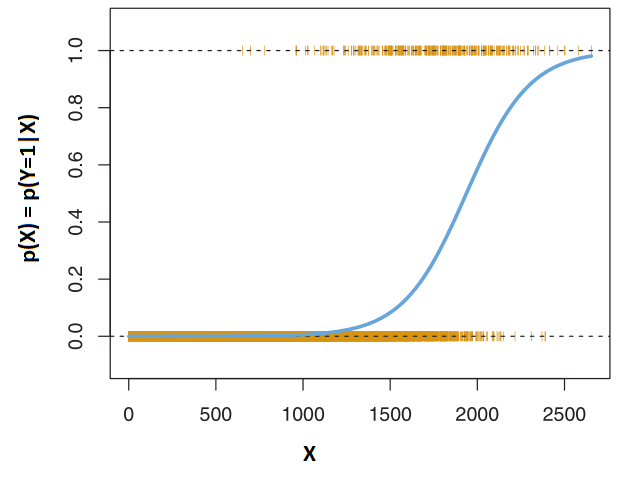
\includegraphics{img/lr_example.png}
\caption{}
\end{figure}

As for prediction, we use the model built with the estimated parameters
to predict probabilities. For example,

If \(X=1000\),

\[ \hat{p}(X) = \frac{e^{\hat{\beta_0} + \hat{\beta_1} X}}{1+e^{\hat{\beta_0} + \hat{\beta_1} X}} = \frac{e^{-10.6513+0.0055 \times 1000}}{1+e^{-10.6513+0.0055 \times 1000}} = 0.006\]

If \(X=2000\),

\[ \hat{p}(X) = \frac{e^{\hat{\beta_0} + \hat{\beta_1} X}}{1+e^{\hat{\beta_0} + \hat{\beta_1} X}} = \frac{e^{-10.6513+0.0055 \times 2000}}{1+e^{-10.6513+0.0055 \times 2000}} = 0.586\]

\section{Multiple Logistic
Regression}\label{multiple-logistic-regression}

We now consider the problem of predicting a binary response using
multiple predictors. By analogy with the extension from simple to
multiple linear regression in the previous chapters, we can generalize
the simple logistic regression equation as follows:

\[ \log( \frac{p(X)}{1-p(X)} ) = \beta_0 + \beta_1 X_1 +  \ldots + \beta_p X_p\]

where \(X=(X_1,\ldots,X_p)\) are \(p\) predictors. The equation above
can be rewritten as

\[ p(X) = \frac{e^{\beta_0 + \beta_1 X_1 +  \ldots + \beta_p X_p}}{1+e^{\beta_0 + \beta_1 X_1 +  \ldots + \beta_p X_p}} \]

Just as in the simple logistic regression we use the maximum likelihood
method to estimate \(\beta_0,\beta_1,\ldots,\beta_p\).

\chapter*{PW 3}\label{pw-3}
\addcontentsline{toc}{chapter}{PW 3}

\section*{Subsection}\label{subsection}
\addcontentsline{toc}{section}{Subsection}

Text

\section*{Subsection}\label{subsection-1}
\addcontentsline{toc}{section}{Subsection}

Text

\chapter{Discriminant Analysis}\label{discriminant-analysis}

\section{Subsection 1}\label{subsection-1-1}

Text

\section{Subsection 2}\label{subsection-2}

Text

\subsection{~Subsection 3}\label{subsection-3}

Text

\chapter*{PW 4}\label{pw-4}
\addcontentsline{toc}{chapter}{PW 4}

\section*{Subsection}\label{subsection-4}
\addcontentsline{toc}{section}{Subsection}

Text

\section*{Subsection}\label{subsection-5}
\addcontentsline{toc}{section}{Subsection}

Text

\chapter{Support Vector Machines}\label{support-vector-machines}

\section{Subsection 1}\label{subsection-1-2}

Text

\section{Subsection 2}\label{subsection-2-1}

Text

\subsection{~Subsection 3}\label{subsection-3-1}

Text

\chapter*{PW 5}\label{pw-5}
\addcontentsline{toc}{chapter}{PW 5}

\section*{Subsection}\label{subsection-6}
\addcontentsline{toc}{section}{Subsection}

Text

\section*{Subsection}\label{subsection-7}
\addcontentsline{toc}{section}{Subsection}

Text

\part{Unsupervised
Learning}\label{part-unsupervised-learning}
\addcontentsline{toc}{chapter}{(PART) Unsupervised Learning}

\chapter{Dimensionality Reduction}\label{dimensionality-reduction}

\section{Subsection 1}\label{subsection-1-3}

Text

\section{Subsection 2}\label{subsection-2-2}

Text

\subsection{~Subsection 3}\label{subsection-3-2}

Text

\chapter*{PW 6}\label{pw-6}
\addcontentsline{toc}{chapter}{PW 6}

\section*{Subsection}\label{subsection-8}
\addcontentsline{toc}{section}{Subsection}

Text

\section*{Subsection}\label{subsection-9}
\addcontentsline{toc}{section}{Subsection}

Text

\chapter{Clustering: Kmeans}\label{clustering-kmeans}

\section{Subsection 1}\label{subsection-1-4}

Text

\section{Subsection 2}\label{subsection-2-3}

Text

\subsection{~Subsection 3}\label{subsection-3-3}

Text

\chapter*{PW 7}\label{pw-7}
\addcontentsline{toc}{chapter}{PW 7}

\section*{Subsection}\label{subsection-10}
\addcontentsline{toc}{section}{Subsection}

Text

\section*{Subsection}\label{subsection-11}
\addcontentsline{toc}{section}{Subsection}

Text

\chapter{Expectation Maximisation}\label{expectation-maximisation}

\section{Subsection 1}\label{subsection-1-5}

Text

\section{Subsection 2}\label{subsection-2-4}

Text

\subsection{~Subsection 3}\label{subsection-3-4}

Text

\chapter*{PW 8}\label{pw-8}
\addcontentsline{toc}{chapter}{PW 8}

\section*{Subsection}\label{subsection-12}
\addcontentsline{toc}{section}{Subsection}

Text

\section*{Subsection}\label{subsection-13}
\addcontentsline{toc}{section}{Subsection}

Text

\chapter*{References \& Resources}\label{references-resources}
\addcontentsline{toc}{chapter}{References \& Resources}

Readings:

\begin{enumerate}
\def\labelenumi{\arabic{enumi}.}
\tightlist
\item
  Tibshirani
\item
  Andrew Ng
\item
  Applied Linear Statistical Models
\item
  Bishop
\end{enumerate}


\end{document}
